\chapter{System Presentation}
\label{sub:page}
\myTop{The chapter presents how the system works from the perspective of the user, which is key knowledge in order to comprehend the \nameref{chap:implementation}. 
The chapter is divided in two sections, one presents the project group \viewroom[] and the other presents the administrative part. }


\section{Project Group Room}
A screenshot of a project group room can be seen in \figref{fig:projectgroupnoedit}. 
In this project group room the blocks of the standard layout are seen.
\begin{figure}[h]
	\centering
		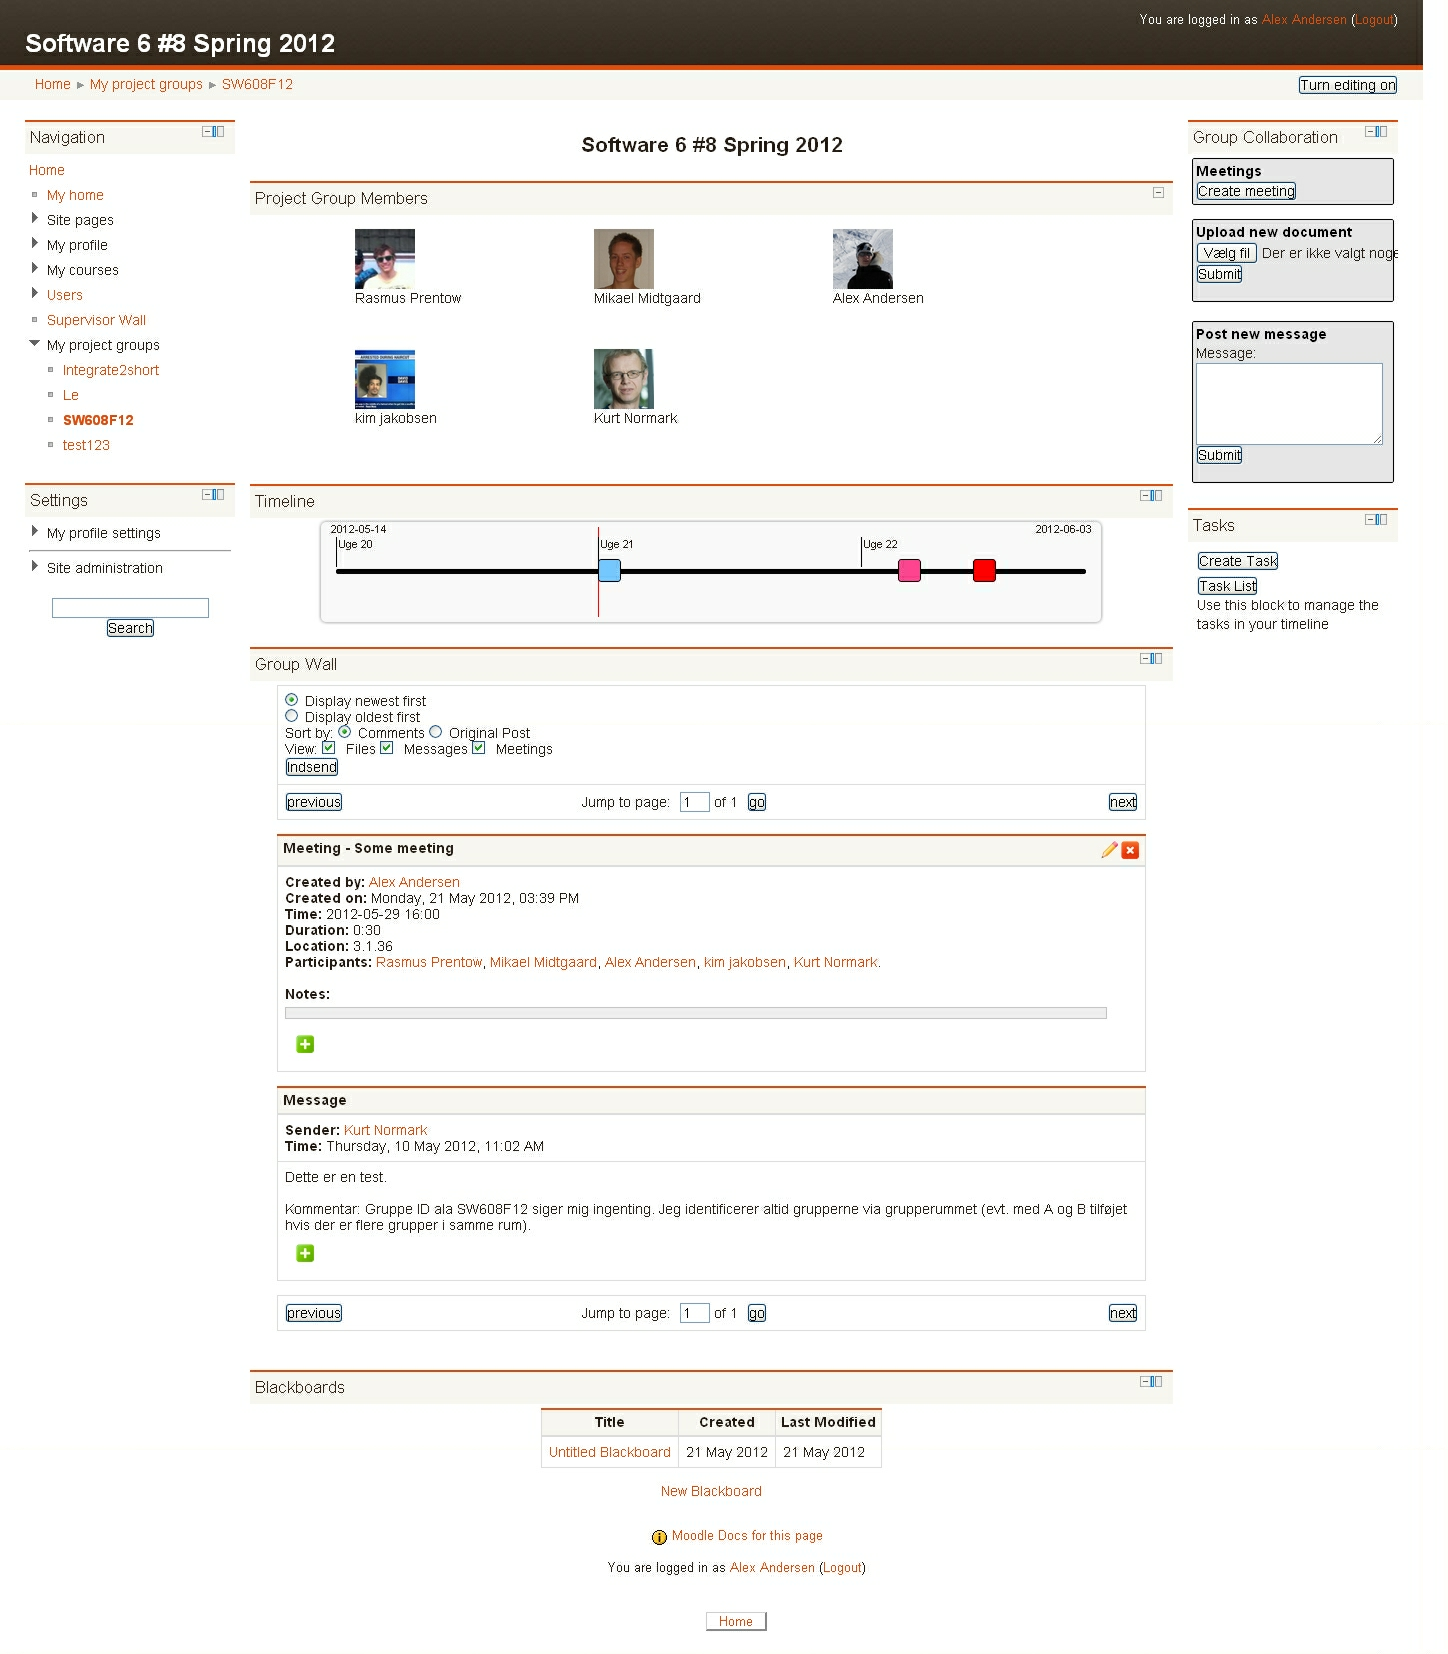
\includegraphics[width=\textwidth]{images/projectgroupnoedit.png}
	\morscaption{The project group room}
	\label{fig:projectgroupnoedit}
\end{figure}

The project group room consist of three columns and three rows. 
The screenshot illustrates the area boundaries by dashed lines. 
%An illustrationThe page in edit mode can be seen in figure \figref{fig:projectgroupwithedit}.
The three rows on the page are: The header, the middle, and the footer. 
%The header is standard Moodle and is only controlled by us to add a heading. 
The header is standard Moodle and we effect it by adding a headline the rest is added automatically.
The heading shows the name of the project group. 
The middle part is the actual project group room it is divided in three columns. 
The left column is the standard navigation menu in Moodle and is not created by us, though it is extended by us.
%We do not want anything to be added to this column to ensure that the page seem familiar to the user.
The center and right columns both contain \block{}s.
The center area is much wider than the left and right and can therefore contain bigger \block{}s. 
The various \block{}s presented on the project groups page are described in \secref{sec:implprojectgroupblocks}. 
If a user wants to edit the layout for the project group room he can press the ``Turn editing on'' button. 
This will allow the user to remove, add, move, and edit \block{}s. 
A special ``add new block''-block is added in editing mode to allow for adding new \block{}s. 
If a user edits the page, the change can be seen by all group members. 

The figure an example of a \block{} can be seen, it is denoted with the grayed out area.
The grayed out area is the members block and is created by our group, we will elaborate on the implementation of this in \secref{sub:membersblock}. 
The block shows a photo and the name of each member of the group. 






\section{Administration}
\label{sec:adminPrensentation}
\todo{Teksten på siden er copyet fra implementationen og skal rettes til}
\todo{Der skal indsæættes SS af edit, og group list. Måske også group members list.}
\todo{Kig evt. på billedet i ovenstaaende section, hvis du syntes det er grimt må du gerne lave det om}
This section presents the system as seen and used by the administrative personnel.

can be accessed through the site administration menu as seen in \figref{fig:navigation}.

\begin{figure}[htb]
	\centering
		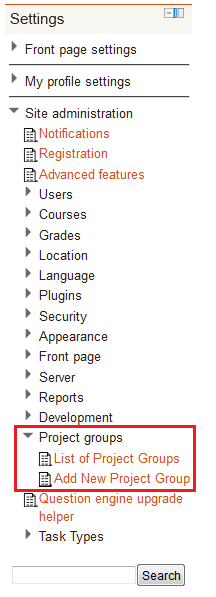
\includegraphics[scale=0.75]{images/admin-navigation.png}
	\morscaption{The settings block, which contains the site administration menu} 
	\label{fig:navigation}
\end{figure}

From here we provide a link to a list of all project groups and a link to a page, from where a new project group can be created.
The page with the list of all project groups has a table with three columns: Short name, Full name, and Actions.
As the name indicates Short name is a short name for a group. 
The Short name also serves as a link to the project group page described in \secref{sub:page}.
In the Actions column there are links to delete and edit the project group.
